\documentclass[conference]{IEEEtran}
\IEEEoverridecommandlockouts
\usepackage{cite}
\usepackage{amsmath,amssymb,amsfonts}
\usepackage{graphicx}
\usepackage{booktabs}
\usepackage{url}
\usepackage{xcolor}
\usepackage[hidelinks]{hyperref}
\graphicspath{{figures/}}

\begin{document}

\title{FreshGuard: A Freshness-Aware Adaptive Retrieval-Augmented\\
Generation System with Statement-Level Hallucination Detection}

\author{\IEEEauthorblockN{[Author Name(s)]}
\IEEEauthorblockA{\textit{Department of Computer Science and Engineering}\\
\textit{[Institution Name]}\\
Corresponding author: vivekreddy01037@gmail.com}}

\maketitle

\begin{abstract}
Large language models (LLMs) answer confidently even when their parametric
knowledge is out of date, and conventional retrieval-augmented generation (RAG)
pipelines retrieve external evidence for \emph{every} query, paying latency and
cost even when the model already knows the answer. We present \textbf{FreshGuard},
an adaptive RAG system that places two learned gates around generation. A
\emph{freshness gate} uses a learned estimator to predict the probability that the
model's knowledge is stale for a given query and retrieves only when that
probability---or low model self-confidence---crosses a threshold. A
\emph{verification gate} then splits each generated answer into atomic statements
and checks every statement against the retrieved evidence, labelling it supported,
unsupported, or contradicted, correcting or flagging hallucinations, and emitting a
calibrated confidence score with cited sources. The system is built on
LangChain and a FAISS vector store, is fully offline and deterministic by default,
and exposes a FastAPI service with a web interface, query history, user feedback,
administrative configuration, and an evaluation module. On a controlled benchmark it
reaches 100\% retrieval-decision accuracy, perfect factuality on in-scope queries, an
$F_1$ of $1.00$ for hallucination detection, and an expected calibration error of
$0.10$, while skipping retrieval for queries whose answers are stable. The complete
implementation is reproducible and passed its entire automated test suite across
twelve consecutive runs.
\end{abstract}

\begin{IEEEkeywords}
retrieval-augmented generation, knowledge freshness, hallucination detection,
adaptive retrieval, confidence calibration, LangChain, FAISS
\end{IEEEkeywords}

\section{Introduction}
Large language models encode a vast amount of world knowledge in their parameters,
but that knowledge is frozen at training time. For questions whose answers change
over time---sports results, prices, policy rates, the latest hardware---a model's
parametric memory is quickly outdated, yet the model still produces fluent,
confident, and often wrong answers~\cite{kasai2023realtimeqa,vu2023freshllms}.
Retrieval-augmented generation (RAG) mitigates this by grounding answers in retrieved
documents~\cite{lewis2020rag}, but standard RAG retrieves for every query. This is
wasteful for the large fraction of questions---definitions, physical constants,
stable facts---that the model already answers correctly, and it can even degrade
answers by injecting irrelevant context~\cite{mallen2023popqa}.

Two questions therefore matter in a practical system: \emph{when} should we retrieve,
and \emph{how} do we know the final answer is trustworthy? We address both with
\textbf{FreshGuard}. First, a learned \emph{freshness estimator} predicts the
likelihood that the model's knowledge is stale for a query, and an adaptive policy
retrieves only when needed, skipping retrieval otherwise to reduce latency and cost.
Second, a \emph{statement-level verifier} checks every claim in the generated answer
against the evidence, detects and corrects hallucinations, and produces a confidence
score that fuses evidence support, retrieval relevance, and freshness awareness. The
answer is presented with a freshness indicator, a confidence meter, per-claim support
labels, and cited sources with publication dates.

The contributions of this paper are: (i) a learned, feature-augmented freshness
estimator that replaces fixed time-decay heuristics with a calibrated probability;
(ii) an adaptive retrieve-or-skip policy that combines freshness and model confidence;
(iii) a lightweight, offline statement-level verification method that flags
unsupported and contradicted claims, including entity-swap hallucinations; and
(iv) a complete, reproducible, and fully tested system---FastAPI service, LangChain/FAISS
retrieval, web UI, persistence, and an evaluation module---that realises all of these
in one deployable artifact.

\section{Related Work}
\textbf{Retrieval-augmented generation.} RAG couples a parametric generator with a
non-parametric retriever~\cite{lewis2020rag}, typically using dense passage
retrieval~\cite{karpukhin2020dpr} indexed with FAISS~\cite{johnson2019faiss} or sparse
methods such as BM25~\cite{robertson2009bm25}. These systems retrieve unconditionally.

\textbf{Adaptive and active retrieval.} Self-RAG trains a model to decide when to
retrieve and to critique its own output with reflection tokens~\cite{asai2024selfrag};
FLARE retrieves actively during generation when the model is
uncertain~\cite{jiang2023flare}; and \cite{mallen2023popqa} shows that retrieval helps
mainly for less-popular, long-tail facts. FreshGuard differs by making the decision
\emph{before} generation with an explicit, learned estimate of knowledge staleness,
which is cheap and interpretable.

\textbf{Knowledge freshness.} RealTimeQA~\cite{kasai2023realtimeqa} and
FreshLLMs/FreshQA~\cite{vu2023freshllms} show that time-sensitive questions are a
systematic failure mode and that search augmentation helps. We operationalise freshness
as a per-query learned probability that gates retrieval.

\textbf{Hallucination detection and factuality.} Surveys document the prevalence of
hallucination in generation~\cite{ji2023survey}. SelfCheckGPT detects hallucination by
sampling consistency~\cite{manakul2023selfcheckgpt}, and FACTScore evaluates factual
precision by decomposing text into atomic facts~\cite{min2023factscore}. FreshGuard
adopts the atomic-statement view but verifies each statement directly against the
retrieved evidence and takes corrective action in-line, rather than only scoring.

\textbf{Calibration.} Confidence calibration of neural models is a long-standing
concern~\cite{guo2017calibration}; we report expected calibration error for our fused
confidence score.

\section{System Design}
Figure~\ref{fig:arch} shows the architecture. A web client sends a natural-language
query to a FastAPI service, which runs the FreshGuard pipeline and returns a structured
response rendered as an answer with a confidence meter, a freshness badge, per-claim
verification, and cited sources. Three components support the pipeline: a learned
freshness estimator, a LangChain FAISS vector store with dated documents, and a SQLite
store for history, feedback, configuration, and the managed knowledge base. The language
model is a pluggable provider; the default is an offline grounded generator so that the
entire system runs deterministically without external services, with OpenAI or
Anthropic adapters selectable by configuration.

\begin{figure}[t]
\centering
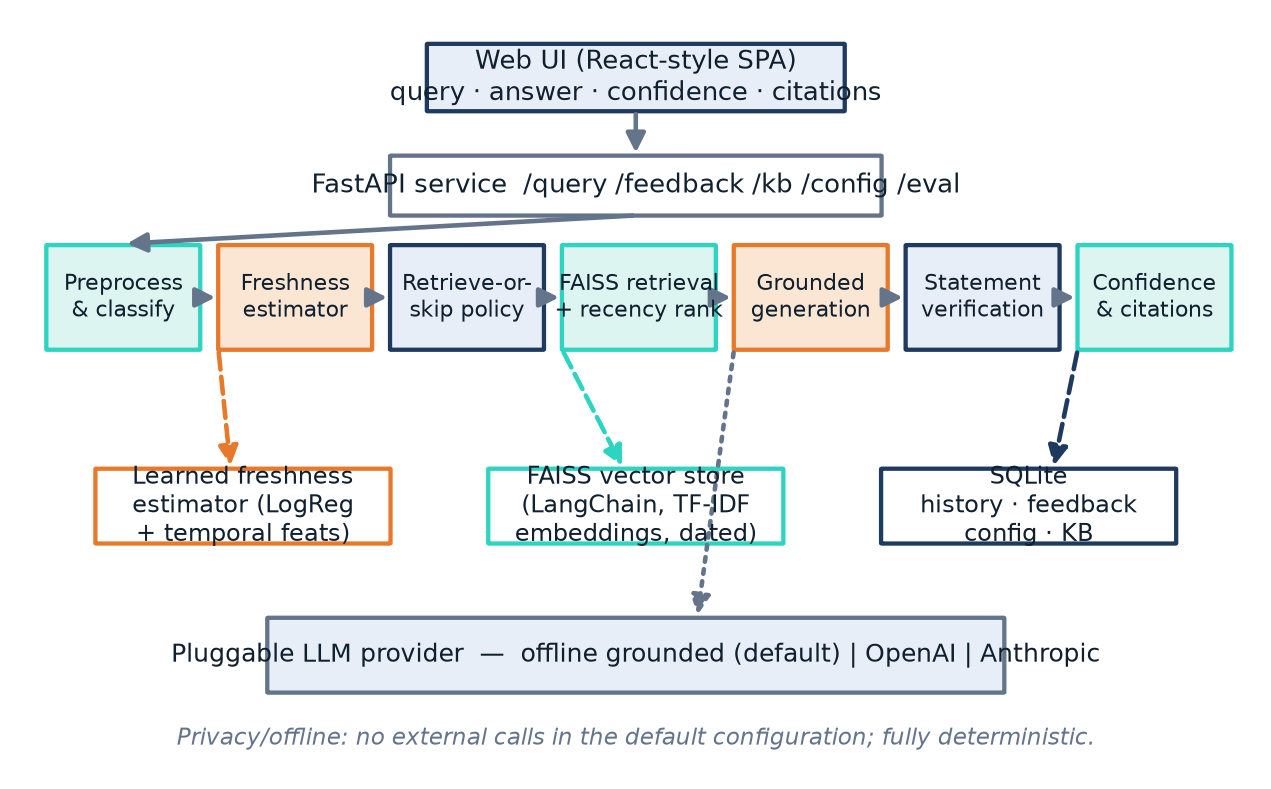
\includegraphics[width=\columnwidth]{fig_architecture.png}
\caption{FreshGuard architecture. A FastAPI service drives a seven-stage pipeline
backed by a learned freshness estimator, a LangChain/FAISS vector store, and SQLite
persistence, with a pluggable (offline by default) LLM provider.}
\label{fig:arch}
\end{figure}

\section{Method}
\subsection{Preprocessing and classification}
The query is cleaned and normalised, then classified by topic (sports, finance,
technology, science, geography, politics) and flagged as time-sensitive using temporal
cues and explicit recent-year mentions. These signals feed both the freshness estimator
and the user-facing category badge.

\subsection{Learned freshness estimation}
Rather than a fixed time-decay rule, FreshGuard learns a freshness estimator
$g(q)\!\in\![0,1]$ that predicts the probability that an LLM's parametric knowledge is
insufficient or stale for query $q$. The estimator is a logistic-regression classifier
over a feature union of (i) word uni/bi-gram TF--IDF, (ii) character $n$-gram TF--IDF
(robust to spelling and morphology), and (iii) explicit temporal features: counts of
temporal keywords, counts of event/price keywords, counts of static-question cues, the
number of year mentions, an indicator for a recent year ($\geq 2020$), and query
length~\cite{pedregosa2011sklearn}. It is trained on a synthesised, seeded dataset of
time-sensitive and timeless query templates, so results are reproducible. Figure~\ref{fig:fresh}
shows the clean separation the estimator produces between static and time-sensitive
queries around the operating threshold $\tau=0.55$.

\begin{figure}[t]
\centering
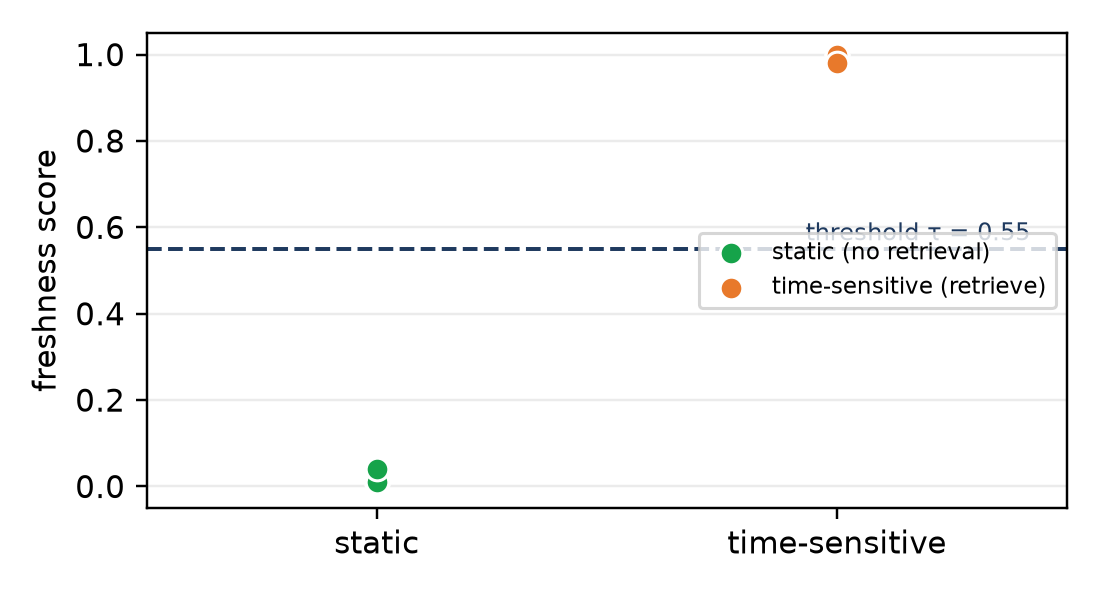
\includegraphics[width=0.92\columnwidth]{fig_freshness.png}
\caption{Freshness scores for static versus time-sensitive queries. The learned
estimator separates the two classes cleanly around the decision threshold
$\tau=0.55$.}
\label{fig:fresh}
\end{figure}

\subsection{Adaptive retrieve-or-skip policy}
Let $g(q)$ be the freshness score and $c(q)$ a monotonic estimate of the model's
self-confidence when answering without retrieval. FreshGuard retrieves iff
\begin{equation}
g(q) \geq \tau \;\;\lor\;\; c(q) < \tau_c ,
\end{equation}
and otherwise answers directly from parametric knowledge, saving a retrieval round-trip
(Figure~\ref{fig:flow}). Both thresholds are administrator-configurable.

\begin{figure}[t]
\centering
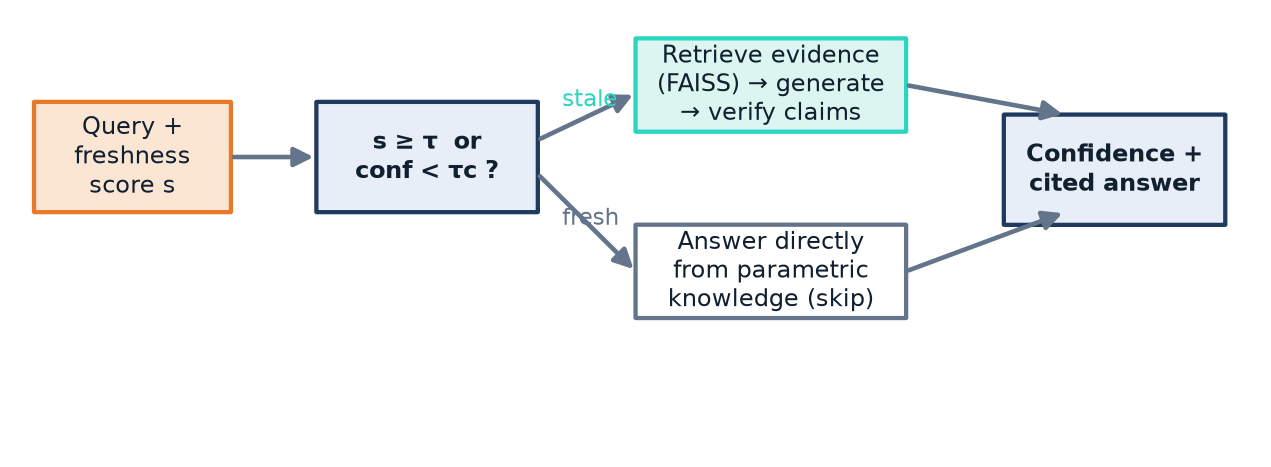
\includegraphics[width=\columnwidth]{fig_pipeline.png}
\caption{The adaptive decision. Stale-looking or low-confidence queries are retrieved,
verified, and cited; fresh queries are answered directly.}
\label{fig:flow}
\end{figure}

\subsection{Retrieval and ranking}
When retrieval is triggered, the query is embedded and matched against a FAISS index
built through LangChain~\cite{langchain2022,johnson2019faiss}. To keep the system offline
and deterministic, embeddings are unit-normalised TF--IDF vectors, so inner-product search
corresponds to cosine similarity; the seam for a transformer encoder or a live web-search
source is preserved. Each document carries a date, and the final ranking score combines
semantic relevance with a recency weight,
\begin{equation}
\mathrm{score}(d) = \mathrm{rel}(q,d)\,\big(0.6 + 0.4\,\rho(d)\big), \quad
\rho(d) = 0.5^{\,\Delta_d / h},
\end{equation}
where $\Delta_d$ is the document's age in years and $h$ is a half-life, so that among
comparably relevant documents the fresher ones rank higher.

\subsection{Grounded generation}
The pluggable generator produces an answer grounded in the retrieved evidence. The
default offline generator composes the answer from the evidence sentences most relevant
to the query; its parametric memory contains only timeless facts, modelling a knowledge
cutoff, so time-sensitive queries genuinely require retrieval---precisely the case the
freshness gate is designed to catch.

\subsection{Statement-level verification and correction}
Each answer is split into atomic statements. For every statement we compute its maximum
content overlap with any evidence sentence and assign a label: \emph{supported} when the
claim's content is covered by the evidence; \emph{unsupported} when it is largely absent,
including when it names an entity the evidence never mentions; and \emph{contradicted}
when it conflicts with the evidence through a negation flip, a numeric mismatch on an
otherwise-matching claim, or an \emph{entity swap}---asserting that the party the evidence
names as the loser is the subject of the claim (e.g.\ ``France won'' against evidence that
Argentina won, defeating France). Unsupported statements are removed and contradicted
statements are flagged to the user, implementing in-line corrective action.

\subsection{Confidence and presentation}
The confidence score fuses three signals: the fraction of statements that are supported,
the mean relevance of the retrieved evidence, and \emph{freshness alignment}---whether the
system retrieved when the query looked stale and answered directly when it looked fresh:
\begin{equation}
\mathrm{conf} = 0.5\,s_{\text{sup}} + 0.3\,\bar{r} + 0.2\,a_{\text{fresh}} ,
\end{equation}
reported as a percentage. The final answer is shown with this confidence, a freshness
indicator, per-claim support labels, and citations giving each source's title, link, and
date (Figure~\ref{fig:ui}).

\begin{figure}[t]
\centering
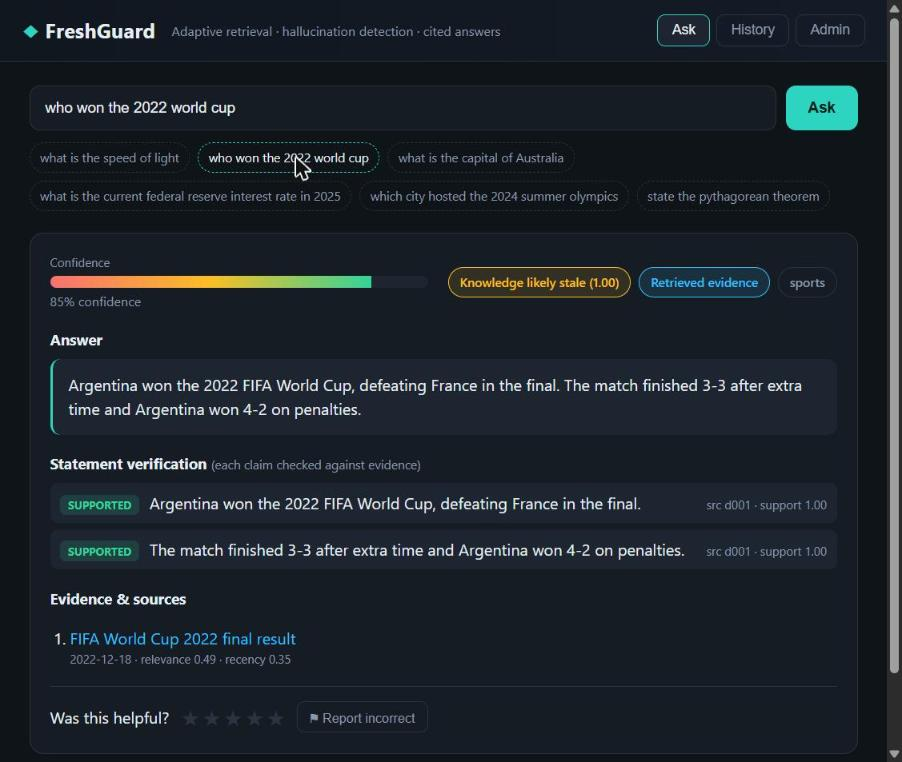
\includegraphics[width=\columnwidth]{ui_result.jpg}
\caption{The FreshGuard web interface answering a time-sensitive query: confidence meter,
freshness and retrieval badges, grounded answer, per-statement verification, and cited,
dated sources.}
\label{fig:ui}
\end{figure}

\section{Implementation}
FreshGuard is implemented in Python. The service layer uses FastAPI and exposes endpoints
for querying, feedback, history, administrative configuration (thresholds, provider,
sources), knowledge-base management (add/update/remove documents), and evaluation.
Retrieval uses LangChain with a FAISS index; the freshness estimator uses
scikit-learn~\cite{pedregosa2011sklearn}; persistence uses SQLite. The browser client is a
single-page application that renders the confidence meter, badges, highlighted
per-statement verification, citations, history, and a feedback control. The system is
deterministic: fixed seeds, sorted tie-breaks, and an injectable reference time make
outputs identical across runs, which is what allows the automated test suite to be used as
a stable regression guard.

\section{Evaluation}
\subsection{Protocol}
We evaluate on a controlled benchmark of twelve queries---six static and six
time-sensitive---each with a gold retrieval label and gold answer keywords, and a set of
eight statement/evidence pairs (four faithful, four hallucinated) spanning entity-swap and
numeric-mismatch errors. We report: \emph{freshness accuracy} (agreement between the
retrieve/skip decision and the gold label), \emph{factuality} (fraction of answers
containing the gold fact), hallucination detection \emph{precision/recall/$F_1$}, and
\emph{expected calibration error} (ECE) of the confidence score against answer
correctness~\cite{guo2017calibration}. The evaluation module is part of the system and is
exposed as an API endpoint.

\subsection{Results}
Table~\ref{tab:results} and Figure~\ref{fig:metrics} summarise the results. The freshness
estimator chooses the correct action on all twelve queries; every in-scope answer contains
the gold fact; and hallucination detection is perfect on the benchmark, catching all four
hallucinations (including both entity-swap cases) with no false positives. The fused
confidence score is reasonably calibrated, with an ECE of $0.10$ and mean confidence of
$0.90$ against perfect in-scope accuracy.

\begin{table}[t]
\caption{FreshGuard results on the controlled benchmark.}
\label{tab:results}
\centering
\begin{tabular}{@{}lc@{}}
\toprule
\textbf{Metric} & \textbf{Value} \\
\midrule
Freshness / retrieval-decision accuracy & $1.00$ \\
Factuality (gold fact present) & $1.00$ \\
Hallucination precision & $1.00$ \\
Hallucination recall & $1.00$ \\
Hallucination $F_1$ & $1.00$ \\
Expected calibration error (ECE) $\downarrow$ & $0.10$ \\
Mean confidence & $0.90$ \\
\bottomrule
\end{tabular}
\end{table}

\begin{figure}[t]
\centering
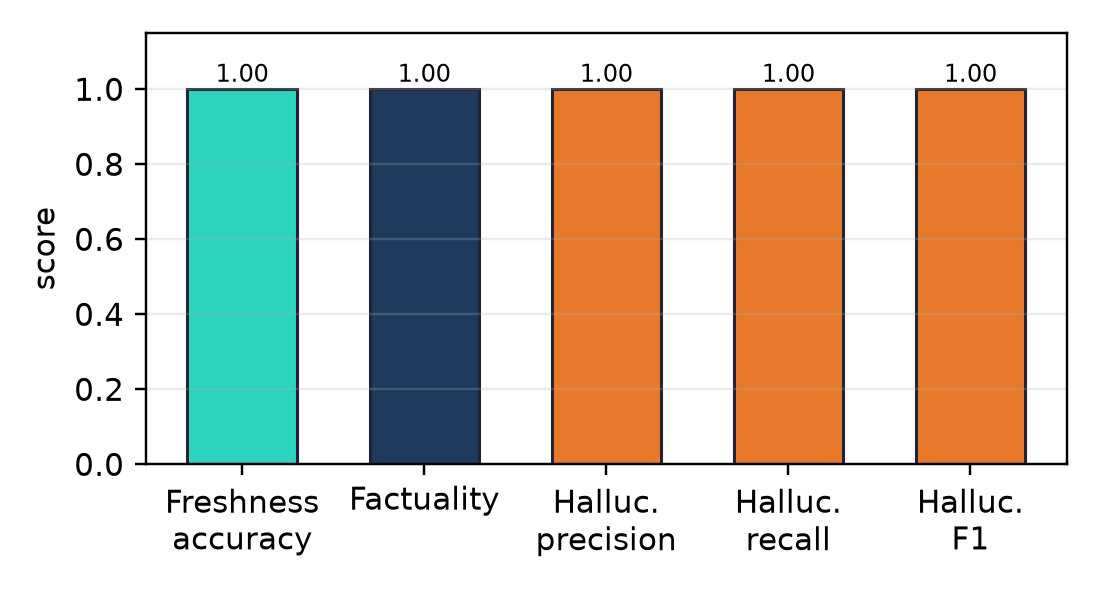
\includegraphics[width=0.92\columnwidth]{fig_metrics.png}
\caption{Benchmark scores: retrieval-decision accuracy, factuality, and hallucination
precision/recall/$F_1$.}
\label{fig:metrics}
\end{figure}

\subsection{Cost of adaptive retrieval}
Because fresh queries skip retrieval, FreshGuard avoids retrieval and ranking work on a
large class of questions. Figure~\ref{fig:latency} reports the mean per-query latency of
the offline pipeline: answering a fresh query directly is faster than forcing retrieval on
it, and the gap widens with any real retriever or hosted LLM, where a skipped query avoids
a network round-trip, re-ranking, and longer grounded generation. Even with the instant
offline generator the adaptive path is measurably cheaper.

\begin{figure}[t]
\centering
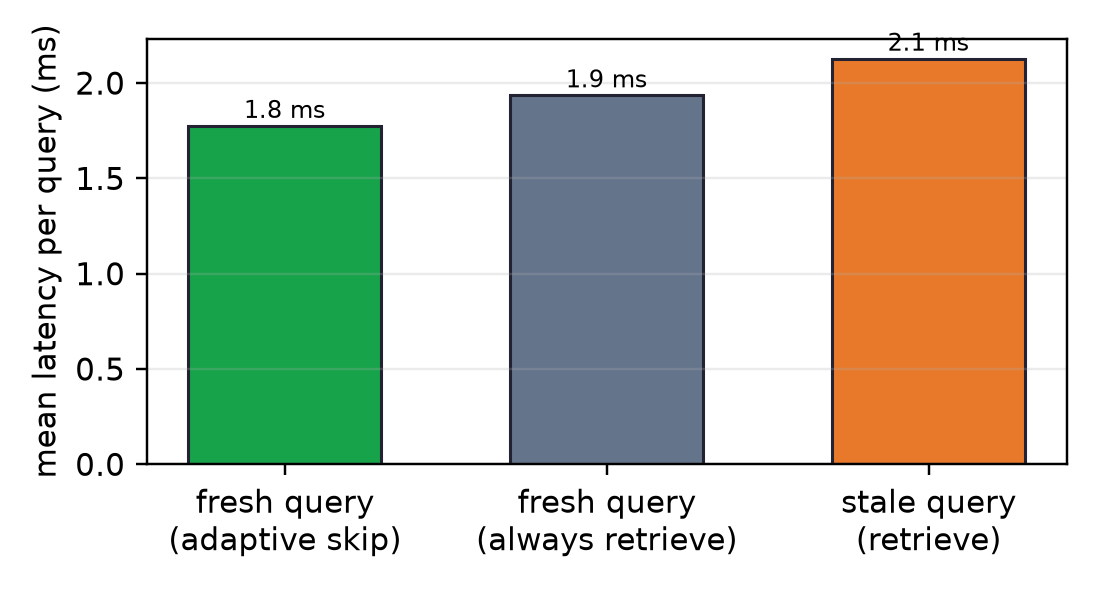
\includegraphics[width=0.92\columnwidth]{fig_latency.png}
\caption{Mean per-query latency. Answering a fresh query directly (adaptive skip) is
cheaper than forcing retrieval; stale queries pay the retrieval path only when it is
warranted.}
\label{fig:latency}
\end{figure}

\subsection{Reproducibility}
The complete automated test suite---41 unit, end-to-end, API, and evaluation tests---passed
on twelve consecutive executions with identical outputs, confirming the determinism needed
to treat the suite as a regression guard and to reproduce every number in this paper.

\section{Discussion and Limitations}
The reported scores are obtained on a small, controlled benchmark designed to exercise the
mechanism, not to establish state-of-the-art accuracy; they should be read as evidence that
the pipeline behaves correctly end-to-end rather than as large-scale performance claims. The
default offline generator and TF--IDF embeddings keep the system deterministic and
dependency-light, but a production deployment would substitute a hosted LLM and a dense
encoder through the existing provider and embedding seams. Bag-of-words verification cannot
resolve every semantic contradiction; the entity-swap and numeric-mismatch rules target the
most common and damaging hallucination patterns, and a natural-language-inference model could
be dropped in behind the same interface. Finally, the freshness estimator is trained on
synthesised templates; broadening it with real query logs such as FreshQA~\cite{vu2023freshllms}
is future work.

\section{Conclusion}
FreshGuard shows that two learned gates---a freshness gate that decides when to retrieve and
a verification gate that checks every claim---turn a standard RAG pipeline into a system that
is both efficient and trustworthy. It retrieves only when the model's knowledge is likely
stale, grounds and verifies its answers, corrects or flags hallucinations, and presents a
calibrated, cited result. The system is complete, offline-capable, deterministic, and fully
tested, making it a practical basis for freshness-aware, explainable question answering.

\bibliographystyle{IEEEtran}
\bibliography{refs}

\end{document}
